

\subsection{Blob-Erkennung mit OpenMV}

{\tiny Quelle: \textcolor{blue}{\url{https://docs.arduino.cc/tutorials/nicla-vision/blob-detection}}}



In diesem Beispiel wird der Arduino Nicla Vision verwendet, um das Vorhandensein und die Position von Objekten in einem Kamerabild zu erkennen. Dazu wird eine Technik verwendet, die als Blob-Erkennung bezeichnet wird. Für diese Aufgabe wird ein MicroPython-Skript erstellt und mit Hilfe der OpenMV IDE auf der Nicla Vision ausgeführt. OpenMV IDE ermöglicht einerseits die Kommunikation mit dem Arduino-Board und andererseits wird auf einfache Weise eine Vorschau des Videostreams anzeigt, so dass Farbbereiche visuell inspiziert werden können, um Schwellenwerte zu definieren. 

\subsection{Blob-Erkennung}

Dieser Blob-Algorithmus \index{Blob-Algorithmus} ermöglicht die Erkennung von Bereichen in einem digitalen Bild, die sich in Eigenschaften wie Helligkeit oder Farbe von den umliegenden Bereichen unterscheiden. Diese Bereiche werden als Kleckse bezeichnet. Stellen Sie sich einen Blob als einen Klumpen ähnlicher Pixel vor.

\bigskip

Anwendungsbeispiele:

\bigskip

\begin{itemize}
  \item Erkennen bestimmter Fahrzeuge, die vor der Kamera vorbeifahren
  \item Erkennen von fehlenden Teilen in einer Montagelinie
  \item Insektenbefall auf Gemüse erkennen
\end{itemize}
  
\subsection{Erstellen des MicroPython-Skripts}\ 
  
Um Kleckse zu finden, muss dem Algorithmus ein Bild von der Kamera vorgelegt werden. Dieser analysiert es dann und gibt die Koordinaten der gefundenen Kleckse aus. Diese Koordinaten werden direkt auf dem Bild angezeigt und mit Hilfe der roten und grünen LED wird angezeigt, ob ein Fleck gefunden wurde.

Um dies zu ermöglichen, wird zunächst eine neue Datei angelegt, indem Sie auf die Schaltfläche \glqq New File\grqq{} in der Symbolleiste auf der linken Seite geklickt wird. In der leeren Datei werden dann zuerst die erforderlichen Module  importiert:

\begin{itemize}
	\item \PYTHON{pyb}
	\item \PYTHON{sensor}
	\item \PYTHON{image}
	\item \PYTHON{time}
\end{itemize}

Dies ist in Listing \ref{OpenMVBlob1-4} dargestellt.

\begin{code}
	\lstinputlisting[language=Python, firstnumber=1,lastline=4]{../../Code/OpenMV/Blob.py}
	\caption[Skript zur Erstellung der Datei \FILE{train.txt}]{Skript zur Erstellung der Datei \FILE{train.txt} mit den Pfaden zu den Trainingsbildern}\label{OpenMVBlob1-4}
\end{code}
	
Anschließend wird der Sensor konfiguriert. Die Konfiguration ist nun so, dass ein Schnappschuss mit der Kamera gemachent wird. Das zugehörige Listing \ref{OpenMVBlob6-11} ist ebenfalls wiedergegeben. Die wichtigsten Funktionen in diesem Ausschnitt sind \PYTHON{set\_pixformat} und \PYTHON{set\_framesize}. Die Kamera, die mit der Nicla Vision geliefert wird, unterstützt RGB 565 Bilder. Daher müssen wir sie über den Parameter \PYTHON{sensor.RGB565} einstellen. \Mynote{Was ist RGB 565?}
Die Auflösung der Kamera muss auf ein Format eingestellt werden, das sowohl vom Sensor als auch vom Algorithmus unterstützt wird. \PYTHON{QVGA} ist ein guter Kompromiss zwischen Leistung und Auflösung und wird daher verwendet.



\begin{code}
	\lstinputlisting[language=Python, firstline=6,lastline=11]{../../Code/OpenMV/Blob.py}
	\caption{Einen Schnappschuss mit der Kamera machen}\label{OpenMVBlob6-11}
\end{code}



Je nachdem, wie die Kamera positioniert wird, sollten die Funktionen \PYTHON{set\_vflip} und \PYTHON{set\_hmirror} eingesetzt werden. Um das Board mit dem USB-Kabel nach unten zu halten, muss  \PYTHON{set\_vflip(True)} aufgerufen werden. Wenn das Bild so angezeigt werden soll, wie es mit Ihren Augen zu sehen ist, muss \PYTHON{sensor.set\_hmirror(True)} aufgerufen werden. Andernfalls würden Elemente im Bild, wie z. B. Text, gespiegelt werden.


%%%%%%%%%%%%%%%%%%%%
%todo hier weiter

\subsection{Festlegen der Farbschwellenwerte}

Um den Blob-Erkennungsalgorithmus mit einem Bild zu füttern, müssen Sie einen Schnappschuss von der Kamera machen oder das Bild aus dem Speicher laden (z. B. von der SD-Karte oder dem internen Flash). In diesem Fall machen Sie einen Schnappschuss mit der Funktion \PYTHON{snapshot()}. Das resultierende Bild muss dann mit Hilfe der Funktion \PYTHON{find\_blobs} in den Algorithmus eingespeist werden. Sie werden feststellen, dass eine Liste von Tupeln an den Algorithmus übergeben wird. In dieser Liste können Sie die LAB-Farbwerte angeben, die in dem Objekt, das Sie verfolgen möchten, hauptsächlich enthalten sind. Wenn Sie z. B. rein rote Objekte auf schwarzem Hintergrund erkennen wollen, wäre der resultierende Farbbereich sehr schmal. Der entsprechende LAB-Wert für reines Rot ist ungefähr (53,80,67). Ein etwas helleres Rot könnte (55,73,50) sein. Der LAB-Bereich wäre also L: 53-55 A: 73-80 B: 50-67. OpenMV bietet ein praktisches Werkzeug, um die gewünschten Farbbereiche zu ermitteln: Threshold Editor. Sie finden ihn in der OpenMV IDE im Menü unter \menu{Tools > Machine Vision > Threshold Editor}. Platzieren Sie das gewünschte Objekt vor der Kamera und öffnen Sie das Werkzeug. Wenn Sie nach dem Ort des Quellbildes gefragt werden, wählen Sie \glqq Frame Buffer\grqq{}. In dem sich öffnenden Fenster sehen Sie einen Schnappschuss der Kamera und einige Schieberegler zur Anpassung der LAB-Farbbereiche. Wenn Sie die Schieberegler verschieben, sehen Sie im Schwarz-Weiß-Bild auf der rechten Seite, welche der Pixel dem eingestellten Farbbereich entsprechen würden. Weiße Pixel kennzeichnen die passenden Pixel. Wie Sie im folgenden Beispiel sehen können, sind die Pixel eines schönen roten Apfels auf braunem Hintergrund sehr schön gebündelt. Sie ergeben meist einen großen Klecks, siehe Abbildung~\ref{OpenMVLab}.


\begin{figure}
	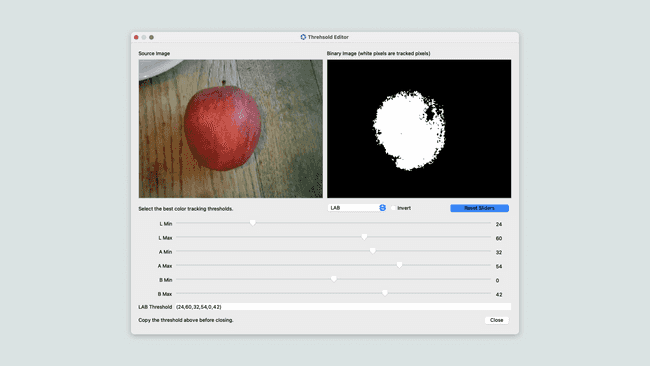
\includegraphics[width=0.8\textwidth]{OpenMV/OpenMVLAB}
	
	\caption{LAB-Schwellenwerte für einen Apfel im Schwellenwert-Editor}
	\label{OpenMVLab}
\end{figure}

Um eine ungefähre Vorstellung vom LAB-Farbbereich des Zielobjekts zu erhalten, können Sie die Histogrammansicht in OpenMV verwenden. Stellen Sie sicher, dass Sie das Histogramm auf den LAB-Farbmodus eingestellt haben. Ziehen Sie mit dem Mauszeiger ein Rechteck direkt über dem Zielobjekt in der Bildpufferansicht auf. Im Histogramm können Sie sehen, welche Farbwerte am häufigsten vorkommen. Sie können die Zielfarbbereiche auf die Minimal- und Maximalwerte der entsprechenden Farbkomponente einstellen.  \ref{OpenMVHisto} 

\begin{figure}
	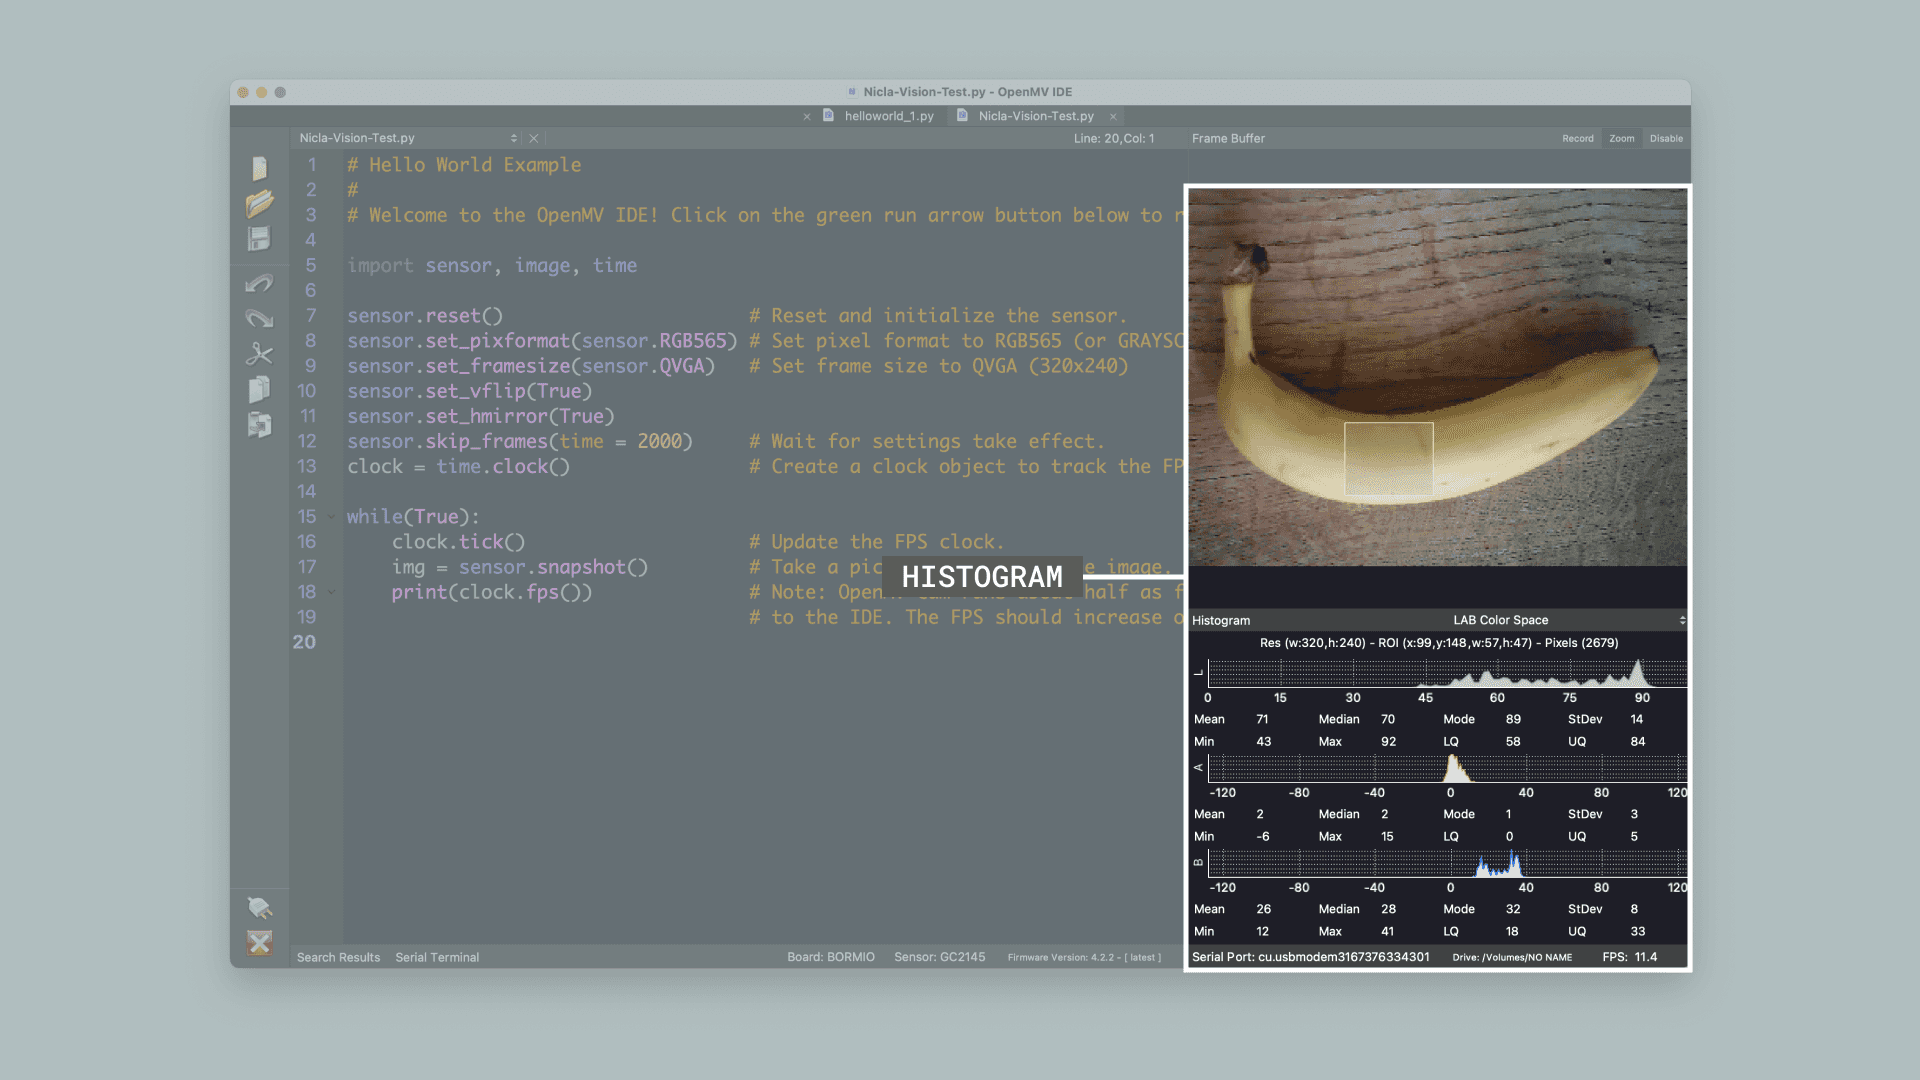
\includegraphics[width=0.8\textwidth]{OpenMV/OpenMVHisto}
	
	\caption{LAB-Farbhistogramm des Bildpuffers}
	\label{OpenMVHisto}
\end{figure}




Im Gegensatz zum obigen Beispiel mit dem Apfel ist die Clusterbildung der Bananenpixel etwas weniger kohärent. Das liegt daran, dass die Banane auf einem Hintergrund liegt, der eine leicht ähnliche Farbe hat. Das bedeutet, dass der Algorithmus empfindlich auf die Hintergrundpixel reagiert. Um Blobs, die nicht zum Zielobjekt gehören, auszuschließen, ist eine zusätzliche Filterung erforderlich. Sie können z. B. eine Mindestgröße des Begrenzungsrahmens (Bounding Box) oder eine Blob-Pixeldichte festlegen, die Dehnung des Objekts oder seine Rundheit definieren oder auch nur nach Objekten in einem bestimmten Teil des Bildes suchen. \ref{OpenMVBanana}


\begin{figure}
	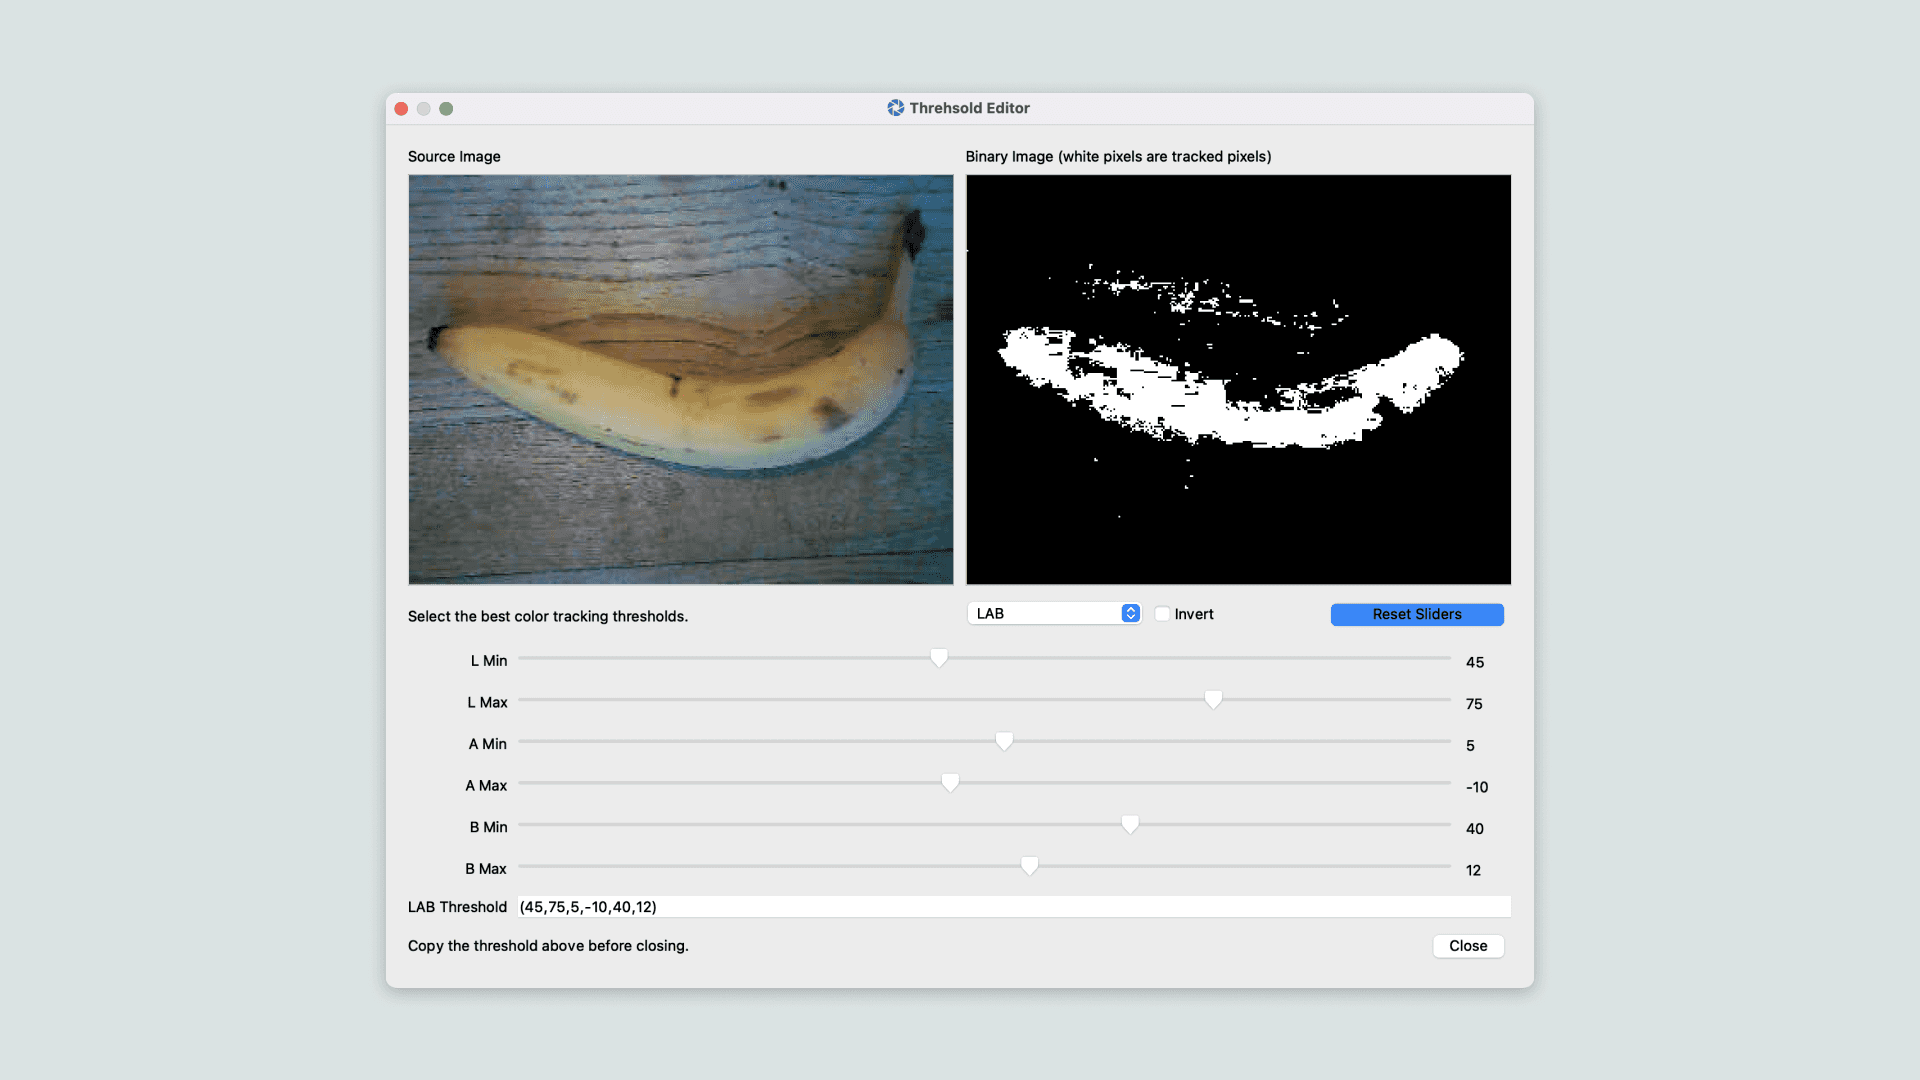
\includegraphics[width=0.8\textwidth]{OpenMV/OpenMVThre}
	
	\caption{LAB-Schwellenwerte für eine Banane im Schwellenwert-Editor}
	\label{OpenMVBanana}
\end{figure}




\subsection{Erkennung von Blobs}

Da Sie nun den Bereich der Farbwerte kennen, der für die Suche nach den Blobs verwendet werden soll, können Sie diese 6 Tupel als Liste an die Funktion \PYTHON{find\_blobs} übergeben \ref{OpenMVBlob13-28}

\begin{code}
	\lstinputlisting[language=Python, firstline=13,lastline=15]{../../Code/OpenMV/Blob.py}

	\lstinputlisting[language=Python, firstline=24,lastline=28]{../../Code/OpenMV/Blob.py}


	\caption{Detektierung von Blobs}\label{OpenMVBlob13-28}
\end{code}


Sobald die Kleckse erkannt sind, möchten Sie vielleicht sehen, wo im Bild sie gefunden wurden. Dies kann durch direktes Zeichnen auf das Kamerabild geschehen, siehe \ref{OpenMVBlob30-35}.


\begin{code}
	
	\lstinputlisting[language=Python, firstline=30,lastline=35]{../../Code/OpenMV/Blob.py}
	
	
	\caption{Anzeigen von Blobs}\label{OpenMVBlob30-35}
\end{code}

Wenn Sie wissen müssen, welcher Blob welcher Farbschwelle entspricht, können Sie die Funktion \PYTHON{blob.code()} verwenden (weitere Informationen finden Sie \href{https://docs.openmv.io/library/omv.image.html#image.image.blob.blob.code}{\textcolor{blue}{hier}}).

Das Ergebnis wird im Frame Buffer-Vorschaufenster auf der rechten Seite der OpenMV-IDE, siehe \ref{OpenMVVisu}, sichtbar sein. 


\begin{figure}
	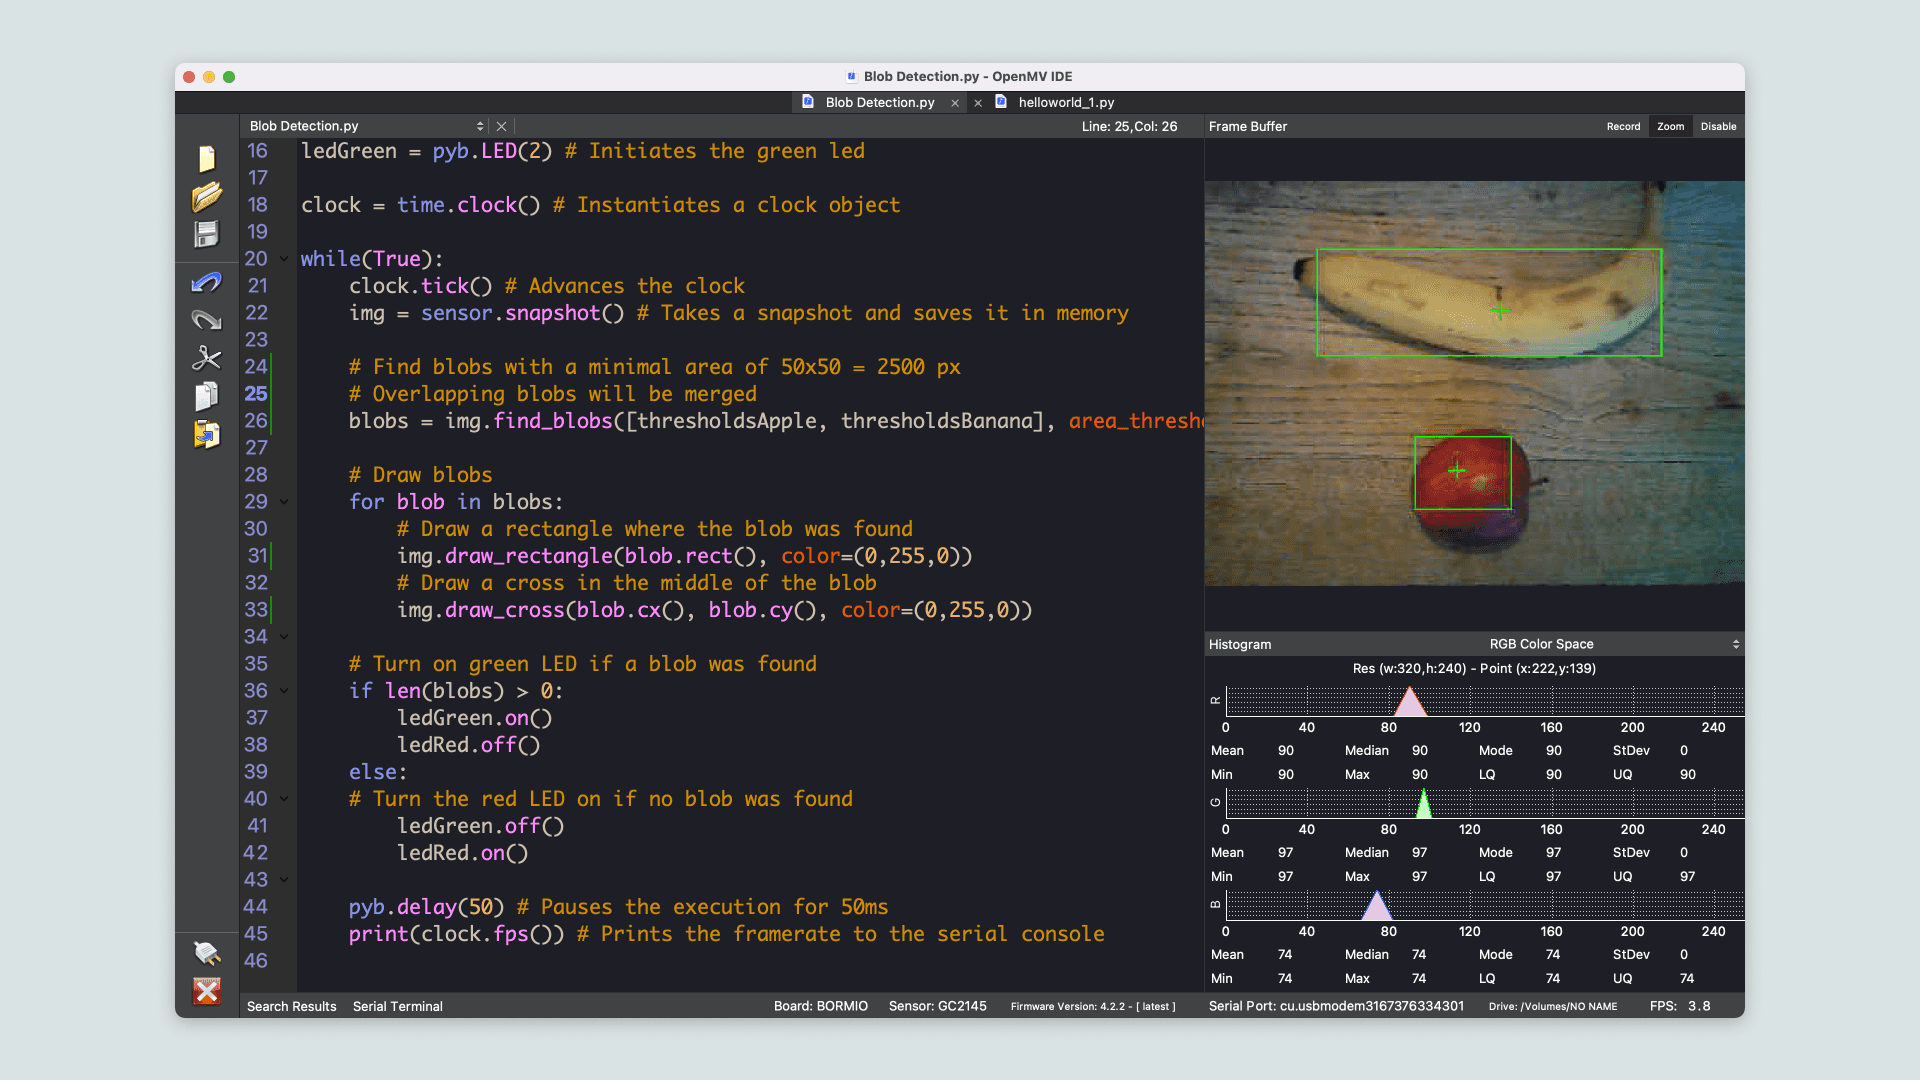
\includegraphics[width=0.8\textwidth]{OpenMV/OpenMVFrame}
	
	\caption{Visualisierung der Blobs in der Bildpuffervorschau}
	\label{OpenMVVisu}
\end{figure}




\subsection{LEDs umschalten}
What if you want some visual feedback from the blob detection without any computer connected to your board? You could use for example the built-in LEDs to indicate whether or not a blob was found in the camera image. Let's initialise the red and the green LEDs with the following code \ref{OpenMVBlob17-18}

\begin{code}
	
	\lstinputlisting[language=Python, firstline=17,lastline=18]{../../Code/OpenMV/Blob.py}
	
	
	\caption{Initialisierung der LEDs}\label{OpenMVBlob17-18}
\end{code}





Fügen Sie dann die Logik hinzu, die die entsprechende LED einschaltet, wenn ein Blob vorhanden ist. Dieser Teil des Codes wird nach der Logik \glqq Draw Blobs\grqq{} hinzugefügt \ref{OpenMVBlob37-44}.




\begin{code}
	
	\lstinputlisting[language=Python, firstline=37,lastline=44]{../../Code/OpenMV/Blob.py}
	
	
	\caption{Initialisierung der LEDs}\label{OpenMVBlob37-44}
\end{code}

In diesem Beispiel leuchtet die grüne LED auf, wenn mindestens ein Blob im Bild gefunden wurde. Die rote LED leuchtet, wenn kein Blob gefunden werden konnte.

\subsection{Hochladen des Skripts}


Programmieren wir das Board mit dem vollständigen Skript und testen wir, ob der Algorithmus funktioniert. Kopieren Sie das folgende Skript \ref{OpenMVBlobProgram} und fügen Sie es in die neue Skriptdatei ein, die Sie erstellt haben.

\begin{code}
	
	\lstinputlisting[language=Python, firstline=1]{../../Code/OpenMV/Blob.py}
	
	
	\caption{Initialisierung der LEDs}\label{OpenMVBlobProgram}
\end{code}

Klicken Sie auf die Schaltfläche \glqq Play\grqq{} unten in der linken Symbolleiste. Legen Sie einige Objekte auf Ihren Schreibtisch und prüfen Sie, ob Portenta bzw. Nicla Vision sie erkennen kann.

\bigskip


\textbf{Achtung:} Das MicroPython-Skript wird nicht kompiliert und in eine eigentliche Firmware eingebunden. Stattdessen wird es in den internen Flash des Boards kopiert, wo es interpretiert und direkt ausgeführt wird.

